\documentclass[a4paper, 11 pt]{article}
\usepackage[left=2cm,text={17cm, 24cm},top=3cm]{geometry}
\usepackage[czech]{babel}
\usepackage[utf8]{inputenc}

\begin{document}

\begin{titlepage}
\begin{center}
\textsc{\Huge Vysoké učení technické v~Brně
Fakulta informačních technologií} \\
\vspace{\stretch{0.2}}
\Huge \textbf{Formální jazyky a prekladače \\ Algoritmy} \\
\vspace{\stretch{0.2}}
\textsc{\Huge Tým 132, varianta II} \\
\vspace{\stretch{0.1}}
\LARGE \textmd{Erik Kelemen - xkelem01 (vedoucí)\\
	Attila Lakatoš - xlakat01 \\
	Patrik Šober - xsober00 \\
	Tomáš Zubrík - xzubri00} \\
\end{center}
\vspace{\stretch{0.4}}
{\LARGE \today}
\end{titlepage}

\section{\textbf{Rozdelení práce}}
TODO..

\section{\textbf{Diagram konečného automatu}}
VERZE 1.0 - HOTOVO 

\section{\textbf{LL-gramatiku, LL-tabulku a precedenční tabulku, které jsou jádrem vašeho syntaktického analyzátoru}}
TODO..

\newpage
\section*{\Huge{\textbf{Diagram konečného automatu}}}
\begin{figure}[H]
	\begin{center}
	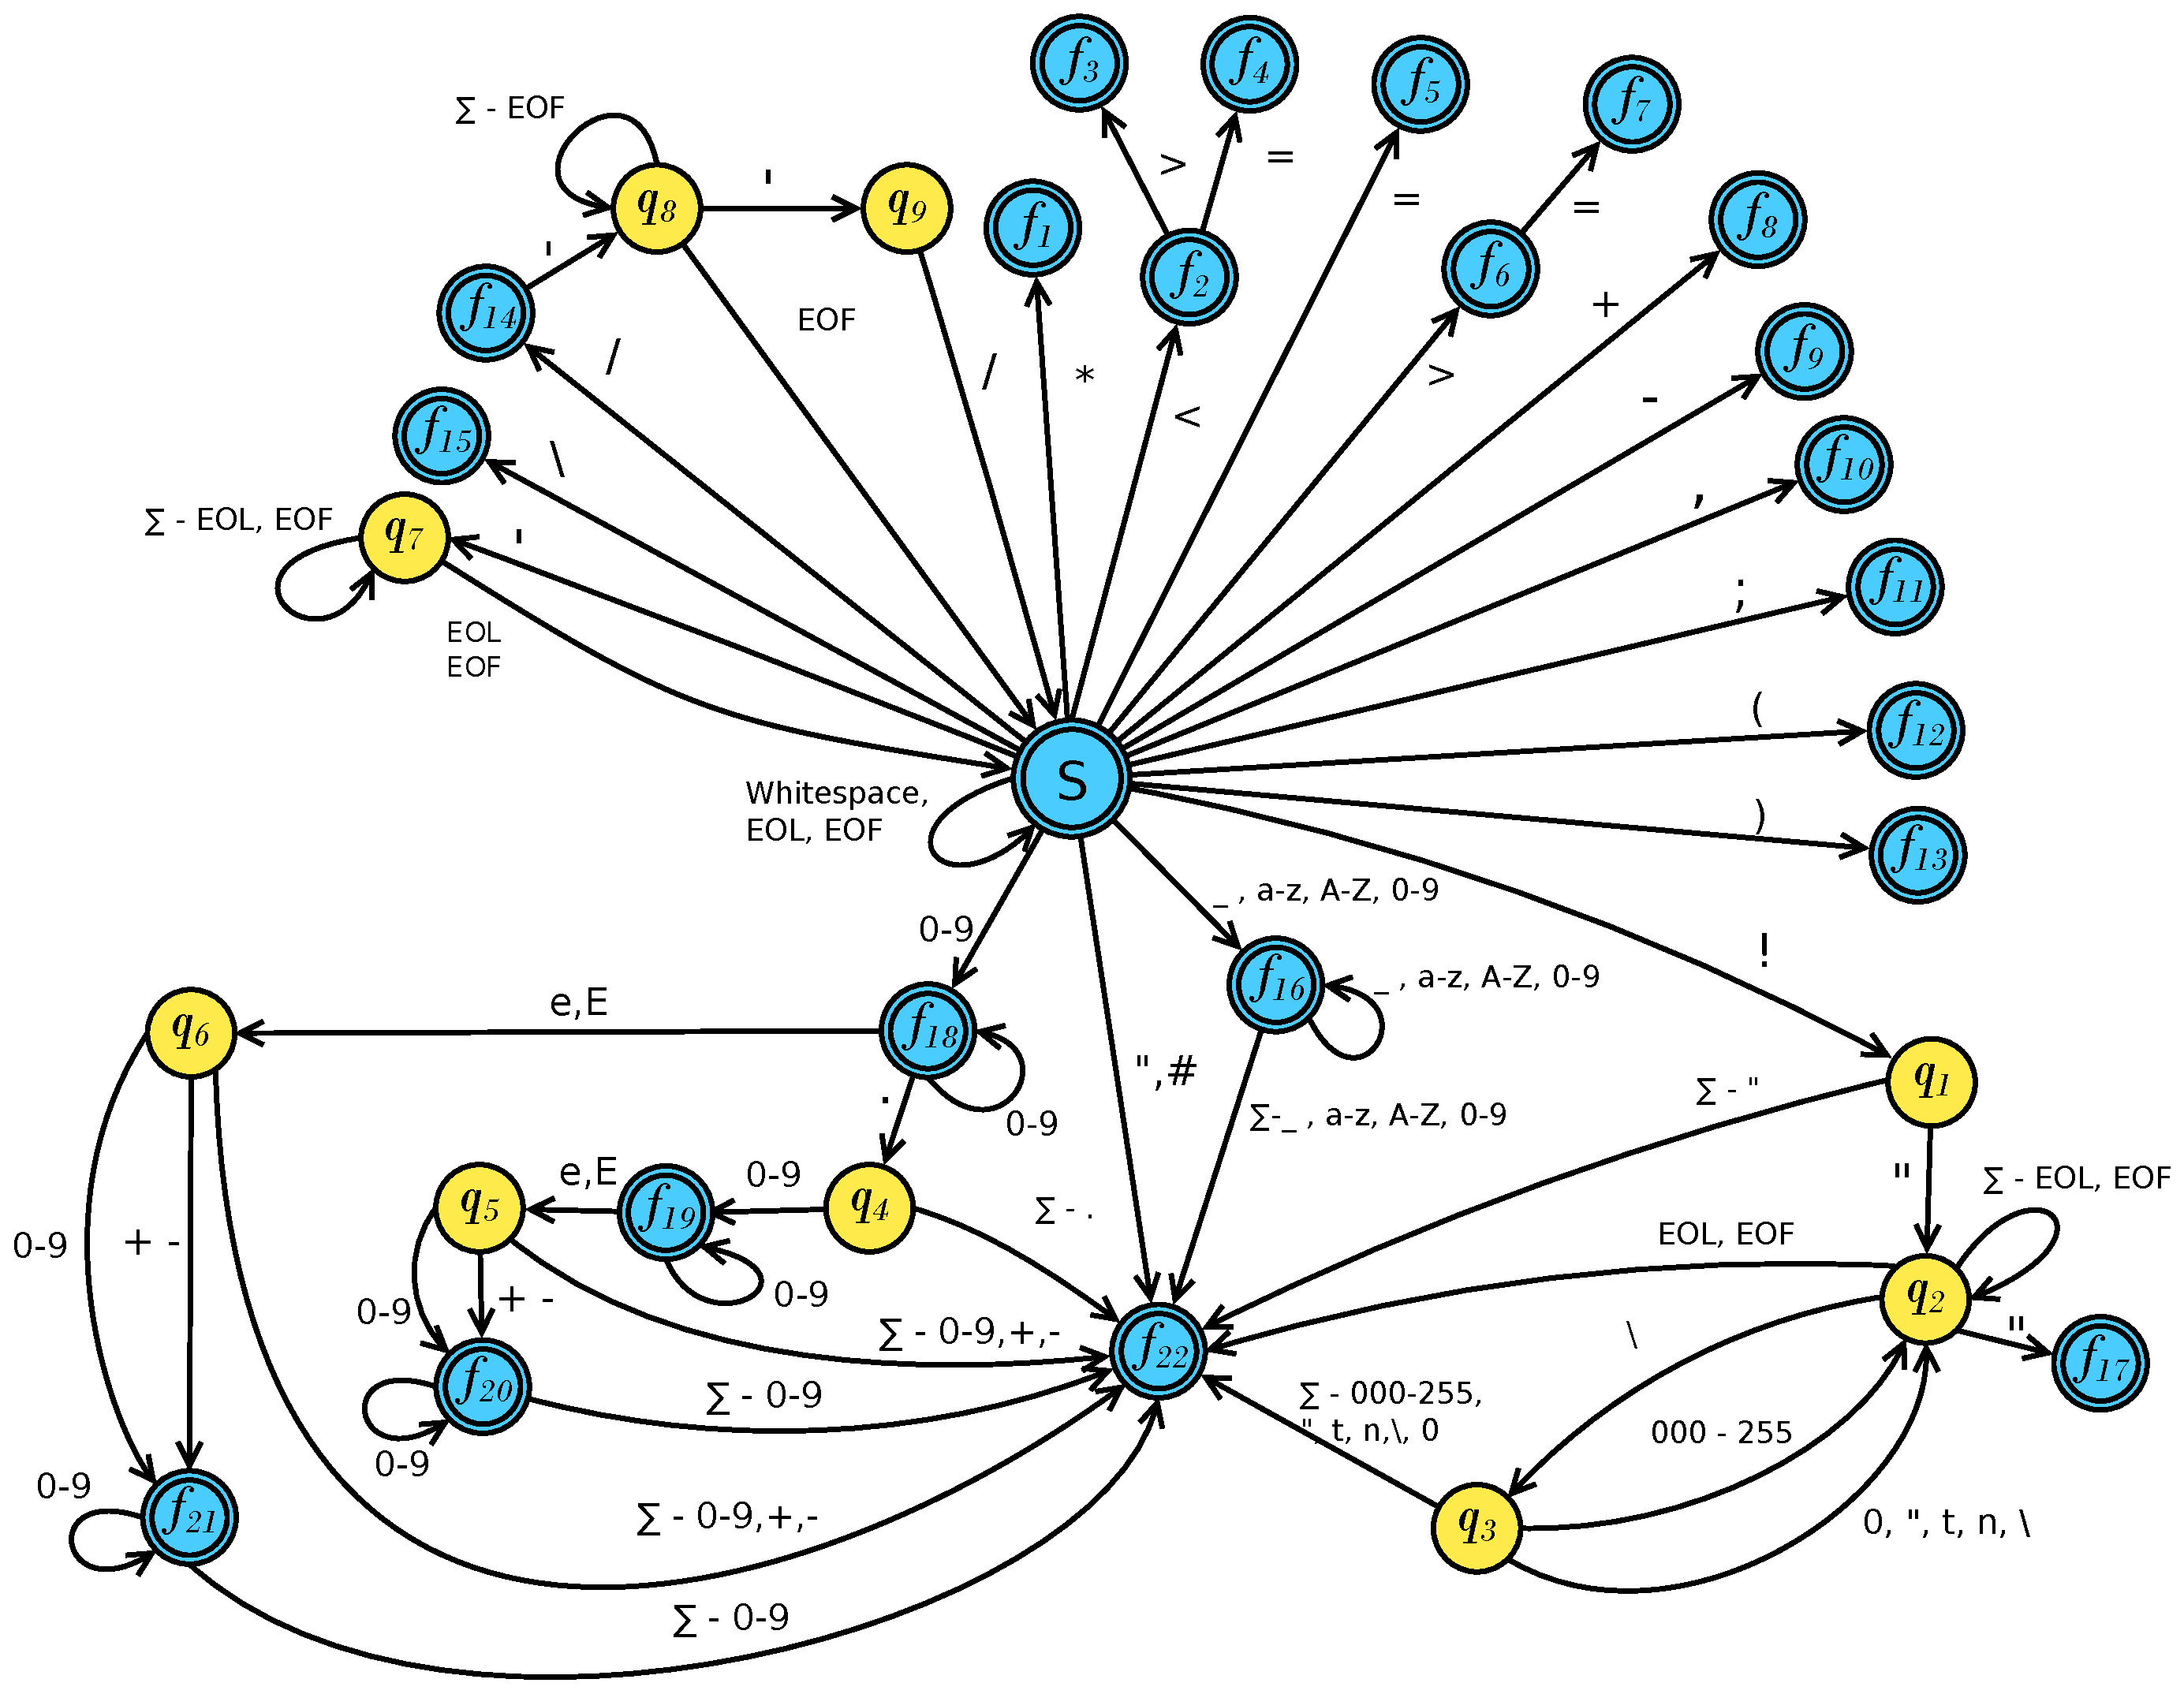
\includegraphics[scale=0.4]{KA_final4.eps}
	\caption{Konečný automat lexikálneho analyzátora}
	\end{center}
\end{figure}
	
\begin{table}[ht]
{
	\renewcommand{\arraystretch}{1.3}
	\begin{center}
		\catcode`\-=12
		\begin{tabular}{| c | l | c | l |} 
		\hline
		\textbf{Označení}  & \textbf{Název stavu}    & \textbf{Označení}  & \textbf{Název stavu}  \\ \hline
		q\textsubscript{1} & EXCLAMATION\_MARK       & q\textsubscript{6} & INT\_EXP              \\ \hline
		q\textsubscript{2} & STRING\_LITERAL\_BEGINS & q\textsubscript{7} & LINE\_COMMENT         \\ \hline
		q\textsubscript{3} & ESCAPE\_SEQUENCE        & q\textsubscript{8} & BLOCK\_COMMENT\_START \\ \hline
		q\textsubscript{4} & DOUBLE\_1               & q\textsubscript{9} & BLOCK\_COMMENT\_END   \\ \hline
		q\textsubscript{5} & DOUBLE\_2               & 			  &                       \\ \hline
		\end{tabular}
	\caption{Konečný automat lexikálneho analyzátora - Stavy}	
	\end{center}
}  
\end{table}
\clearpage
	
\newpage
\thispagestyle{plain}
\begin{table}[!ht]
{
	\renewcommand{\arraystretch}{1.3}
	\begin{center}
		\catcode`\-=12
		\begin{tabular}{| c | l | c | l |} 
		\hline
		\textbf{Označení}   & \textbf{Název stavu}             & \textbf{Označení}   & \textbf{Název stavu}  \\ \hline
		S                   & START,COMMENT,WHITESPACE,EOF,EOL & f\textsubscript{12} & LEFT\_PARANTHESIS     \\ \hline
		f\textsubscript{1}  & MUL                              & f\textsubscript{13} & RIGHT\_PARANTHESIS    \\ \hline
		f\textsubscript{2}  & LESS\_THAN                       & f\textsubscript{14} & DIV     		     \\ \hline
		f\textsubscript{3}  & NOT\_EQUALS                      & f\textsubscript{15} & DIV2                  \\ \hline
		f\textsubscript{4}  & LESS\_OR\_EQUALS                 & f\textsubscript{16} & IDENTIFICATOR         \\ \hline
		f\textsubscript{5}  & EQUALS                           & f\textsubscript{17} & STRING\_LITERAL       \\ \hline
		f\textsubscript{6}  & GREATER\_THAN                    & f\textsubscript{18} & INTEGER               \\ \hline
		f\textsubscript{7}  & GREATER\_OR\_EQUALS              & f\textsubscript{19} & DOUBLE                \\ \hline
		f\textsubscript{8}  & ADD                              & f\textsubscript{20} & DOUBLE\_WITH\_EXP     \\ \hline
		f\textsubscript{9}  & SUB                              & f\textsubscript{21} & INT\_WITH\_EXP        \\ \hline
		f\textsubscript{10} & COMA                             & f\textsubscript{22} & LEXICAL\_ERROR        \\ \hline
		f\textsubscript{11} & SEMICOLON                        &		     & 	     		     \\ \hline
		\end{tabular}
	\caption{Konečný automat lexikálneho analyzátora - Konečné stavy}	
	\end{center}
}  
\end{table}
\clearpage

\end{document}
